%!TEX root =  ../main.tex

\subsection{Anti-Derivative}

\objective{Distinguish and find anti-derivatives and integrals of functions}


Suppose we are given a formula and are told it is the derivative of what we want.
This isn't as abstract as it sounds: velocity is the derivative of position, and (at least in 
many cars) it is easier to record velocity than it is position.  If the velocity
function is an algebraic equation, we simply need to apply the Power Rule
in reverse and we will have the anti-derivative of the equation.

The Power Rule states that the derivative of $x^n$ is $n\cdot x^{n-1}$.  In other words,
``take the exponent out front, and lower the exponent by one''.  If we wanted to
turn this backwards, in order to arrive at an exponent of $x^n$, we must have 
begun at $x^{n+1}$.  However, if we take the derivative of $x^{n+1}$, we must
multiply by $n+1$.  To cancel that, we should multiply by $\frac{1}{n+1}$.


\begin{derivation}{Backwards Power Rule}\index{Power Rule!Backwards}
The anti-derivative of $x^n$ is $\frac{1}{n+1} x^{n+1} + C$, where $C$ is an unknown
constant.
\end{derivation}


What is C?  Consider whether of not $x^2 +1$ is the anti-derivative of $\frac{1}{2}x$.
Is $x^2-1$?  Is $x^2+\pi$?  Because constants differentiate to 0, a constant could be 
part of our anti-derivative equation and we cannot know what it is, without more information.
What information?  Well, if we know the initial conditions (when $x=0$) then we can 
solve for $C$ and know precisely which anti-derivative equation we want.


\subsection{Integral}\index{integral!definite}
The preceding definition of anti-derivatives is very helpful algebraically, but what about
graphically?  If a given graph is the derivative of what we seek, can we interpret the
graph to give us numerical information?

Consider the graph of a car with constant velocity:

\begin{figure}[h]
\begin{centering}
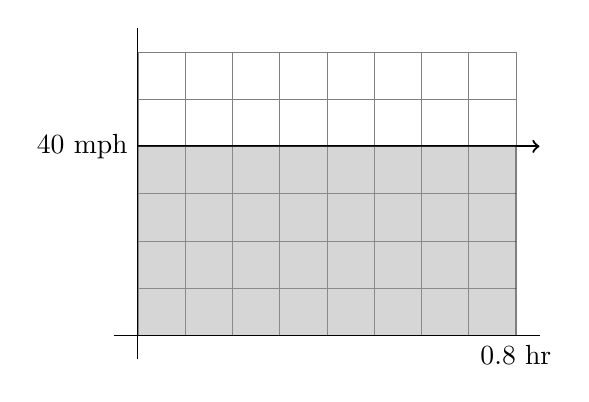
\begin{tikzpicture}[scale=0.6]
	\draw[help lines] (0,0) grid (8,6);
	\draw (-0.5,0) -- (8.5,0);
	\draw (0,-0.5) -- (0,6.5);
	\draw[thick,->] (0,4) node[anchor=east] {40 mph}-- (8.5,4);
	\draw (8,0) node[anchor=north] {0.8 hr};
	\draw [fill=gray!80,opacity =0.4] (0,0) rectangle (8,4);
\end{tikzpicture}
\caption{A car's velocity in 10's of mph, over tenths of an hour}
\end{centering}
\end{figure}


If we want position or distance, we have known a formula for a long time:
distance = rate $\cdot$ time.  The $y$-value is the rate.  The $x$-value is the 
time.  As hard as it may be to conceive of, distance is the \emph{area} under the
graph.  In this case, 40 mph times 0.8 hours is 32 miles.   Notice that this number does
not depend upon the initial position: the car has travelled 32 positive miles, regardless 
of where it began.

\begin{equation}
\int_0^{0.8}  40dx = \left.40x \right|_0^{0.8} = 40(.8) - 40(0) = 32
\end{equation}

What about more complicated velocity?  Let us begin with constant acceleration:

\begin{figure}[h]
\begin{centering}
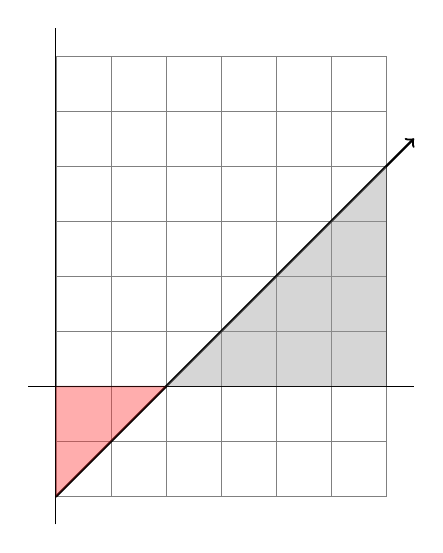
\begin{tikzpicture}[scale=0.7]
	\draw[help lines] (0,-2) grid (6,6);
	\draw (-0.5,0) -- (6.5,0);
	\draw (0,-2.5) -- (0,6.5);
	\draw [thick,->] (0,-2) -- (6.5,4.5);
	\draw [fill=red!80,opacity=0.4] (0,-2) -- (2,0) -- (0,0);
	\draw [fill=gray!80,opacity=0.4] (2,0) -- (6,0) -- (6,4);
\end{tikzpicture}
\caption{A car beginning at -20 mph but steadily accelerating to 40 mph by 0.6 hours later}
\end{centering}
\end{figure}

The object begins with a negative velocity, so we must count that distance as negative.
-2 + 8 = 6, so the object has gained that many units in positive displacement from 0 to 6.

In some problems, we can simply count the squares below the graph and find the
definite integral.  In most cases, the graph will be curved and we will need to find an
anti-derivative equation and subtract the evaluation at the left from that of the right.

Finally, notice that we can integrate functions we cannot differentiate, at times.  It would
be impossible for a physical object to have a velocity graph like the \texttt{int()} function,
but it can still be meaningful to find the area under the graph.

\begin{example}{Bandwidth Rates}
\exProblem
Suppose an wifi hotspot charges start at 2.50 per hour when you begin, and the rate goes
up .50 every 20 minutes after that.  The rate is not incremented
continuously, but jumps every 1/5 hour.  Illustrate the cost of using the service for 0.9 hours
as a definite integral.

\exSolution
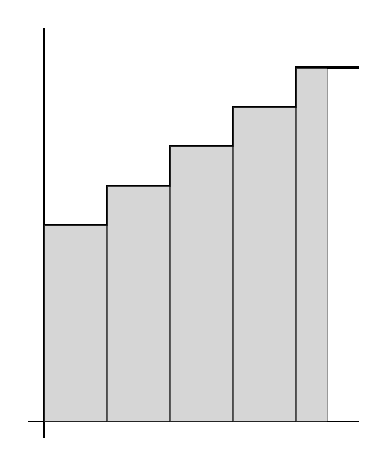
\begin{tikzpicture}[xscale=4,yscale=1]
	\draw (-0.05,0) -- (1,0) ;
	\draw (0,-.2) -- (0,5.0);
	\draw[thick] (0,2.50) -- (.2,2.5) -- (.2,3) -- (.4,3) -- (.4,3.5) -- (.6,3.5) -- (.6,4) -- (.8,4) -- (.8,4.5) -- (1,4.5);
	\draw [fill=gray!80,opacity=0.4] (0,0) rectangle (.2,2.5);
	\draw [fill=gray!80,opacity=0.4] (.2,0) rectangle (.4,3);
	\draw [fill=gray!80,opacity=0.4] (.4,0) rectangle (.6,3.5);
	\draw [fill=gray!80,opacity=0.4] (.6,0) rectangle (.8,4);
	\draw [fill=gray!80,opacity=0.4] (.8,0) rectangle (.9,4.5);
\end{tikzpicture}
As the rectangle illustrate, $(0.2)(2.5) + (0.2)(3.0) + (0.2)(3.5) + (0.2)(4.0) + (0.1)(4.5) = 3.05$.
\end{example}

